\section{Preliminary Results}

The TorCoin protocol does add a small amount of overhead to the Tor traffic. In our experimental setup, we set up a series of servers using the Python Twisted framework to simulate the passing of TorCoin generation and verification messages through a set of relays. 

The total overhead from one round of successful TorCoin mining (i.e., one entire round trip from client through all the relays and back again) results in a total TorCoin packet overhead of 540 bytes. This can be broken down into: 
\begin{itemize}
\item The initial three attempts by each relay: 42 bytes
\item Verification message from Relay 3 to Relay 2: 74 bytes
\item Verification message from Relay 3 to Relay 2: 138 bytes
\item Verification message from Relay 3 to Relay 2: 202 bytes
\end{itemize}

Each round of TorCoin generation and verification happens only after n Tor packets have been sent. Each standard Tor cell is 514 bytes long, so each round trip on the network requires transmission of 514 * 6 = 3084 bytes. Thus, if n > 10, the TorCoin protocol overhead is less than 2\%. The value of n can be calibrated in further experimentation and as needed in order to achieve the sweet-spot of transmission efficiency and incentive maximization for relay providers.

Indeed, one can envision a tunable system where the value of n decreases during times of high usage to incentivise relay providers to temporarily provide more servers to the network.

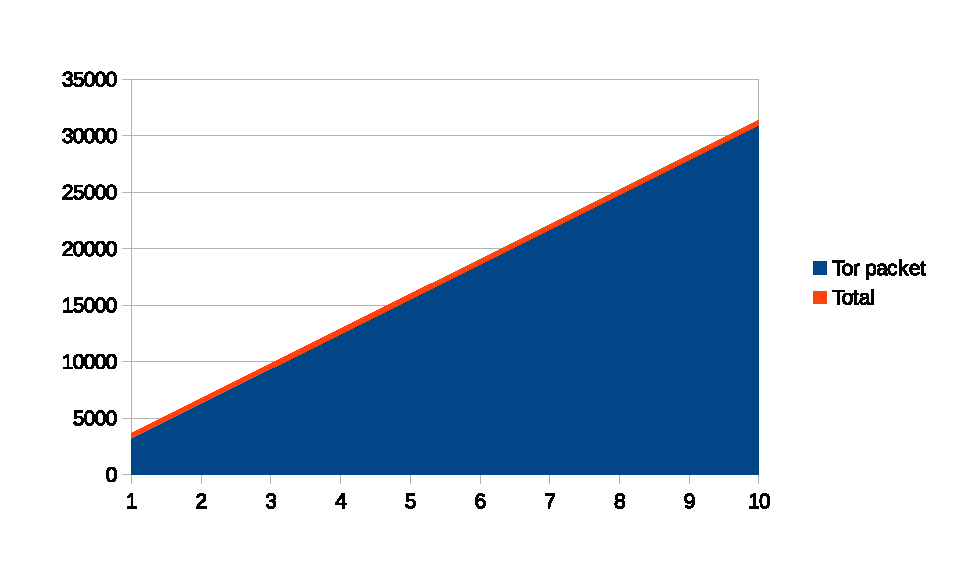
\includegraphics{absolute.eps}

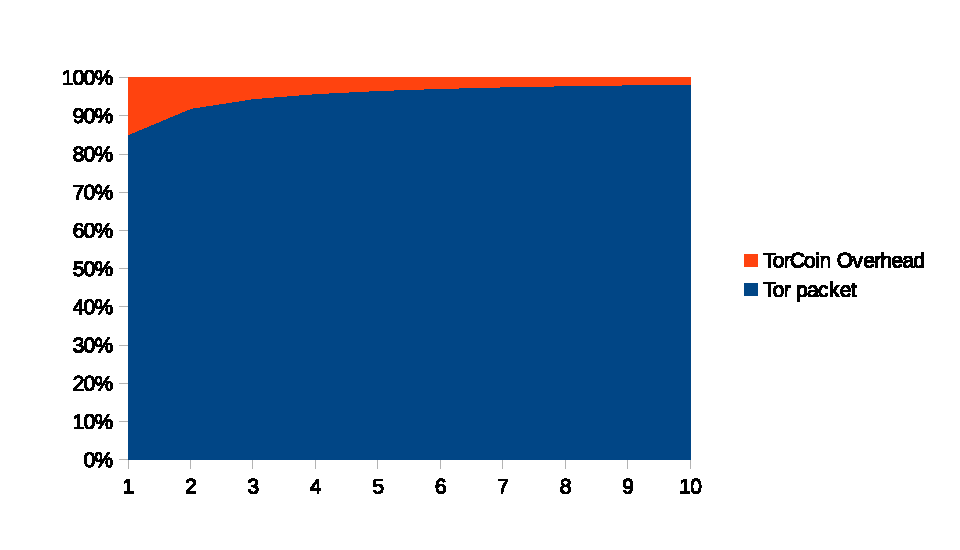
\includegraphics{stacked.eps}

While the Neff shuffle is complicated and requires a large number of communications between all of the servers, in practice, since the number of directory servers that will be involved in each shuffle will be relatively small (less than 10) and are relatively fast servers with high-bandwidth connections with each other, this will not be a major bottleneck. In addition, since this is a one-time cost of connecting to the network, the users will be willing to wait for the slight time that it takes to setup the protocol, especially if the speeds increase sufficiently.